\chapter{序論}
\section{背景}
農業従事者の高齢化や後継者不足などによって作業者の負担が増加しているため, 作業の機械化や自動化が期待されている. 
特に生産の場ではない畦道での草刈り作業は小型機械を背負うなどして人力での作業が行われており, 雑草の成長が著しく高温である夏季に繰り返し行わなければならない重労働である. 
また農地内での荷物の運搬を人力で行う際には農作業一輪車が使われており, 畦道などの細く不安定な道での重量物の運搬は容易とは言い難い. 
これらのように農業には生産活動以外にも従事者の負担となる作業も多くある.  

そのなかで作業負担を減らすための手段のひとつとして移動ロボットの活用が考えられる. 
移動ロボットが自動で畦道を走行することにより荷物の運搬や草刈り作業を自動化をできることや, 
走行する際に畦道上の雑草に対して上から圧力を加えることで雑草の成長の抑制も期待できる\cite{稲垣栄洋2017踏圧処理が畦畔雑草植生に及ぼす影響}. 
このように移動ロボットが畦道を走行することによって様々な作業負担を減らすことが可能であると考えた. 
\begin{figure}[htbp]
\begin{center}
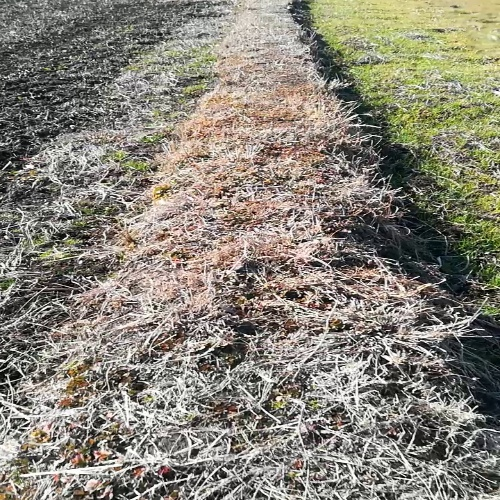
\includegraphics[width=60mm]{figs/fig1.jpg}
\caption{}
\end{center}
\end{figure}

しかし, これらの例を実現するには様々な問題がある.  
例えば図 1.1のように畦道と水田には明確な境界がないために検出が困難であり, 走行箇所である畦道から外れてしまう恐れがあることや, 
傾斜から水田に滑り落ちる可能性があるなどの問題があげられる. 
そのため移動ロボットが自動で畦道を走行するためには, 安全に走行することができる路面を検出する必要がある.



%@@@草ぼうぼうのあぜみちの写真とかがあると説得力出ますね. 

\section{従来研究}

%@@@全体的に読点が少ないような気がします. 
畦道と水田の間には白線や縁石などのような目印となる物がなく, 土を盛り上げているだけであり境界が曖昧である. 
そのため自動運転などに用いられている白線などを基準とした走行箇所の選定を行うことができない. 
そこで畦道上では路面の状態をニューラルネットワークを用いて判別し, 
走行箇所の選定を行う研究\cite{長橋孝哉2019ニューラルネットワークを用いた畦道の雑草検出に関する研究}がある.  
%%%%「路面の検出に関しては」はざっくりしすぎ. 

この研究では畦道上の雑草領域を走行箇所としており, 入力された画像を格子状に雑草領域と路面の二つのクラスに分類している. 
単眼カメラから得た画像をR, G, BとH, S, Vの平均値と分散を特徴量としてニューラルネットワークを用いて学習し分類を行い,   
雑草領域の分類に成功している. しかし, 色の類似した物に対しての誤認識が起きることが課題となっている.

この手法を用いることで畦道上での走行路面の検出をすることは可能だが, 実際に畦道上を移動ロボットが走行するのに用いるのは不十分であると考えた. 
例えば図 1.2のように畦道と水田部の色が似ていることもあり, 走行箇所ではない水田部を走行箇所である畦道と誤認識することが予想される.  
\begin{figure}[htbp]
\begin{center}
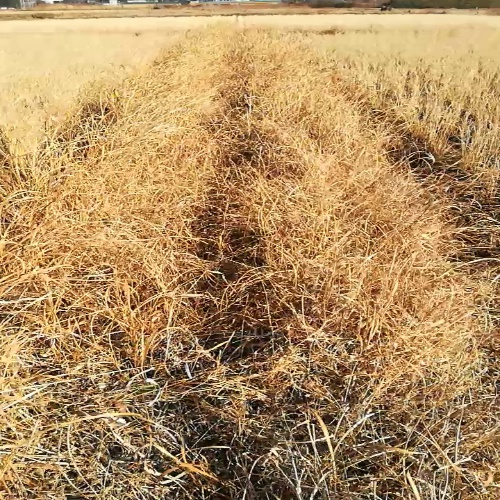
\includegraphics[width=60mm]{figs/fig2.jpg}
\caption{}
\end{center}
\end{figure}
\\また路面の領域の分類のみにとどまっていることから, 走行する際に傾斜や段差のような障害を避けることが難しく, 水田へ滑落することや障害物への接触などが考えられる. 

そのため, 畦道上を移動ロボットが安全に走行できる路面の検出の際には, 走行箇所である畦道領域の取得に加えて傾斜や段差のような障害を回避している必要がある. 
また畦道領域の取得の際には似たような色でも誤認識が起きにくい手法を取り入れる必要がある. 
%@@@!!!!!!!!!!!!!!!だから何???????次のパートにつながらない. 
%%%%草ぼうぼうのあぜみちの写真とかがあると説得力出ますね. 
\section{研究の目的}
本研究では畦道における移動ロボットの安全な走行路面の検出を目的とする. 
移動ロボットが畦道上を走行する際に, 傾斜部や凹凸部などの走行に適さない路面上を通過することで水田への落下などが考えられる. 
そのため,    
\begin{quote}
 \begin{itemize}
  \item 走行箇所である畦道上から外れていない路面であること. 
  \item 傾斜や段差などの障害を考慮した路面であること. 
 \end{itemize}
\end{quote}
以上のことを満たした路面を安全な走行路面とし, 安全な走行路面を検出できる手法の提案および作成を行う. 
%@@@ちゃんと段落分けしましょうね. 参考: https://b.ueda.tech/?post=02586

% dvipdfmxとhereのテスト
%\begin{figure}[H]
%	\begin{center}
%		
\includegraphics[width=1.0\linewidth]{../zero.png}
%		\caption{}
%		\label{fig:}
%	\end{center}
%\end{figure}
%
